
%\documentclass[mathserif]{beamer}
\documentclass[handout]{beamer}
%\usetheme{Goettingen}
\usetheme{Warsaw}
%\usetheme{Singapore}



%\usetheme{Frankfurt}
%\usetheme{Copenhagen}
%\usetheme{Szeged}
%\usetheme{Montpellier}
%\usetheme{CambridgeUS}
%\usecolortheme{}
%\setbeamercovered{transparent}
\usepackage[english, activeacute]{babel}
\usepackage[utf8]{inputenc}
\usepackage{amsmath, amssymb}
\usepackage{dsfont}
\usepackage{graphics}
\usepackage{cases}
\usepackage{graphicx}
\usepackage{pgf}
\usepackage{epsfig}
\usepackage{amssymb}
\usepackage{multirow}	
\usepackage{amstext}
\usepackage[ruled,vlined,lined]{algorithm2e}
\usepackage{amsmath}
\usepackage{epic}
\usepackage{epsfig}
\usepackage{fontenc}
\usepackage{framed,color}
\usepackage{palatino, url, multicol}
%\algsetup{indent=2em}
\newcommand{\factorial}{\ensuremath{\mbox{\sc Factorial}}}
\newcommand{\BIGOP}[1]{\mathop{\mathchoice%
{\raise-0.22em\hbox{\huge $#1$}}%
{\raise-0.05em\hbox{\Large $#1$}}{\hbox{\large $#1$}}{#1}}}
\newcommand{\bigtimes}{\BIGOP{\times}}
\vspace{-0.5cm}
\title{Tackling fairness, change and polysemy in word embeddings}
\vspace{-0.5cm}
\author[Felipe Bravo Márquez]{\footnotesize
%\author{\footnotesize  
 \textcolor[rgb]{0.00,0.00,1.00}{Felipe Bravo-Marquez}} 
  
 
%\vspace{-0.3cm}
\institute{Department of Computer Science, University of Chile \\ National Center for Artificial Intelligence Research \\ Millenium Institute Foundational Research on Data }

\titlegraphic{
\includegraphics[scale=0.06]{pics/logodcc.png}
\includegraphics[scale=0.02]{pics/cenialogo.jpg} 
\includegraphics[scale=0.4]{pics/imfdlogo.png}
\includegraphics[scale=0.15]{pics/RELELA.png}}



\date{\today}

\begin{document}
\begin{frame}
\titlepage


\end{frame}


\begin{frame}{Word Embeddings}
\begin{scriptsize}
\begin{itemize}
\item The first step in computationally working with written language is to represent words as mathematical objects  we can operate with.

\item Representing words as numeric vectors a.k.a \textbf{embeddings} is a standard practice in \textbf{Natural Language Processing} (NLP).

\item Word embeddings are a mapping of discrete symbols (i.e., words) to continuous vectors.


\item Distance between vectors can be equated to distance between words.
\item This makes easier to generalize the behavior from one word to another.

\item Word embeddings have become a core component of natural language processing (NLP) downstream systems (e.g., sentiment analysis, machine translation, question answering).


\end{itemize}
\end{scriptsize}
\end{frame}


\begin{frame}{Word Embeddings}
\begin{figure}[h]
  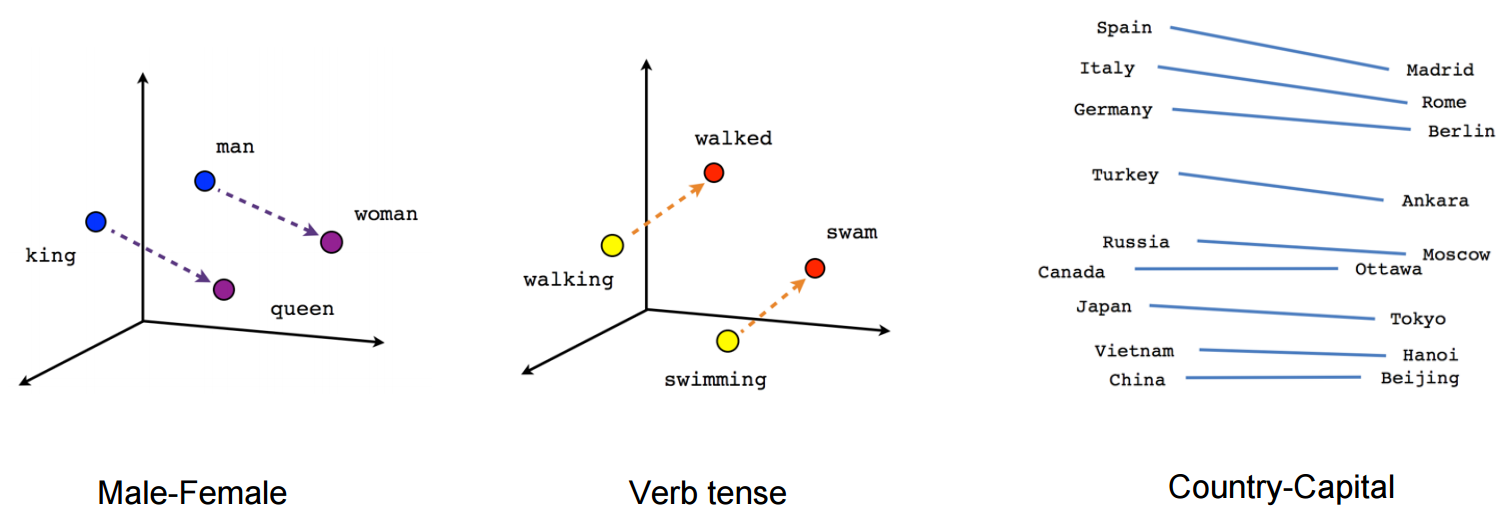
\includegraphics[scale=0.2]{pics/embeddings.png}
\end{figure}
Word embeddings can encode semantic and syntatic relationships between words.


\end{frame}




\begin{frame}{Distributional Hypothesis}
\begin{scriptsize}
\begin{itemize}
\item The construction of word embeddings from document corpora is based on the  \textbf{Distributional Hypothesis} \cite{harris1954}:
\begin{quote}
 Words occurring in the same \textbf{contexts} tend to have similar meanings.
\end{quote}

\item Or equivalently:
\begin{quote}
A word is characterized by the \textbf{company} it keeps.
\end{quote}


\item The idea is to map words occuring in similar contexts to similar vectors.

\end{itemize}
\end{scriptsize}
\end{frame}


\begin{frame}{Word Embeddings}
\begin{figure}[h]
  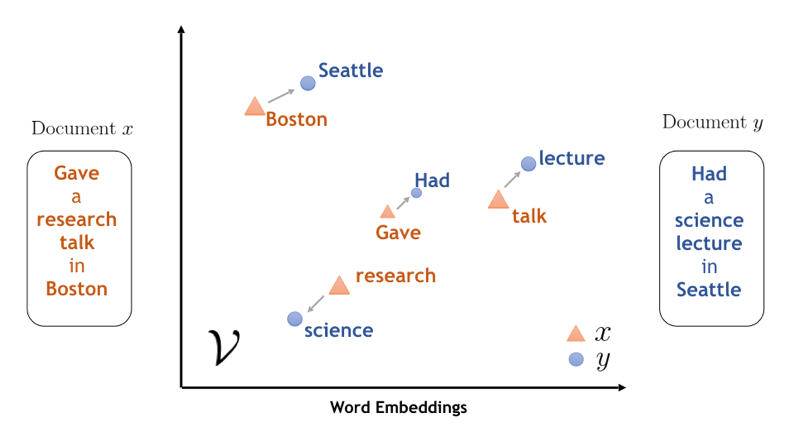
\includegraphics[scale=0.8]{pics/embeddings2.png}
\end{figure}



\end{frame}



\begin{frame}{Word Embeddings Algorithms}
\begin{scriptsize}
\begin{itemize}
\item Word embeddings are build by training neural networks architectures on document corpora (e.g., books, papers, Wikipedia, tweets, the Web).

\item These arquitectures formulate a predictive task (e.g., predict a missing word withing a contex window) in which word embeddings naturally arise from the network's parameters after training.

\item Most popular models are:
\begin{itemize}
\scriptsize{
\item Skip-gram negative sampling \cite{Mikolov2013}
\item Continuous bag-of-words \cite{Mikolov2013}
\item Glove \cite{penningtonSM14}
\item FastText \cite{bojanowski2016enriching}.}
\end{itemize}




\end{itemize}
\end{scriptsize}
\end{frame}

\begin{frame}{Skip-gram Model}

  \begin{figure}[h]
        	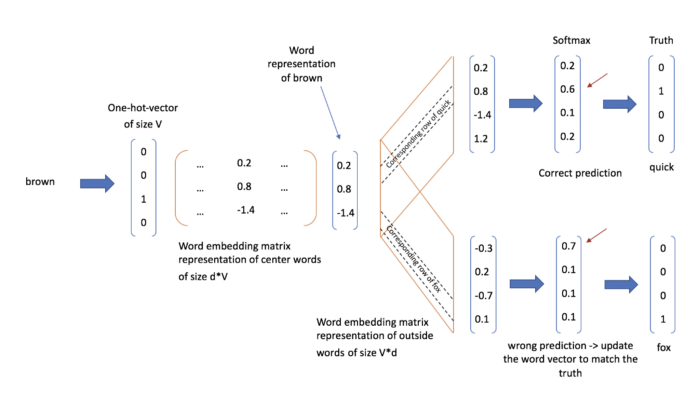
\includegraphics[scale = 0.4]{pics/skip_gram_net_arch.png}
        \end{figure}
\footnotetext{Picture taken from:    \url{http://mccormickml.com/2016/04/19/word2vec-tutorial-the-skip-gram-model/}}

\end{frame}


\begin{frame}{Limitations of Word Embeddings}
\begin{scriptsize}
\begin{itemize}


\item However they suffer from three major limitations:

\begin{enumerate} \scriptsize{
 \item \textbf{Fairness}: they are prone to inherit stereotypical social biases from the corpus they were built on.
 \item \textbf{Change}: they are static. Thus they ignore words not observed during training and are unable to capture semantic drifts.
 \item \textbf{Polysemy}: they fail to capture the polysemous nature of many words (e.g., apple:company, apple:fruit), conflating their multiple senses into a single point.
}
\end{enumerate}


\item In this talk we will present our research addressing these three problems.

\end{itemize}
\end{scriptsize}
\end{frame}



\begin{frame}{WEFE: The Word Embeddings Fairness Evaluation Framework}
\begin{scriptsize}
\begin{itemize}
 \item The Word Embeddings Fairness Evaluation (WEFE) is a framework for measuring and mitigating bias in word embeddings (e.g. man is to programmer as woman is to housewife). \cite{badilla2020wefe}.
\end{itemize}
  \begin{figure}[h]
        	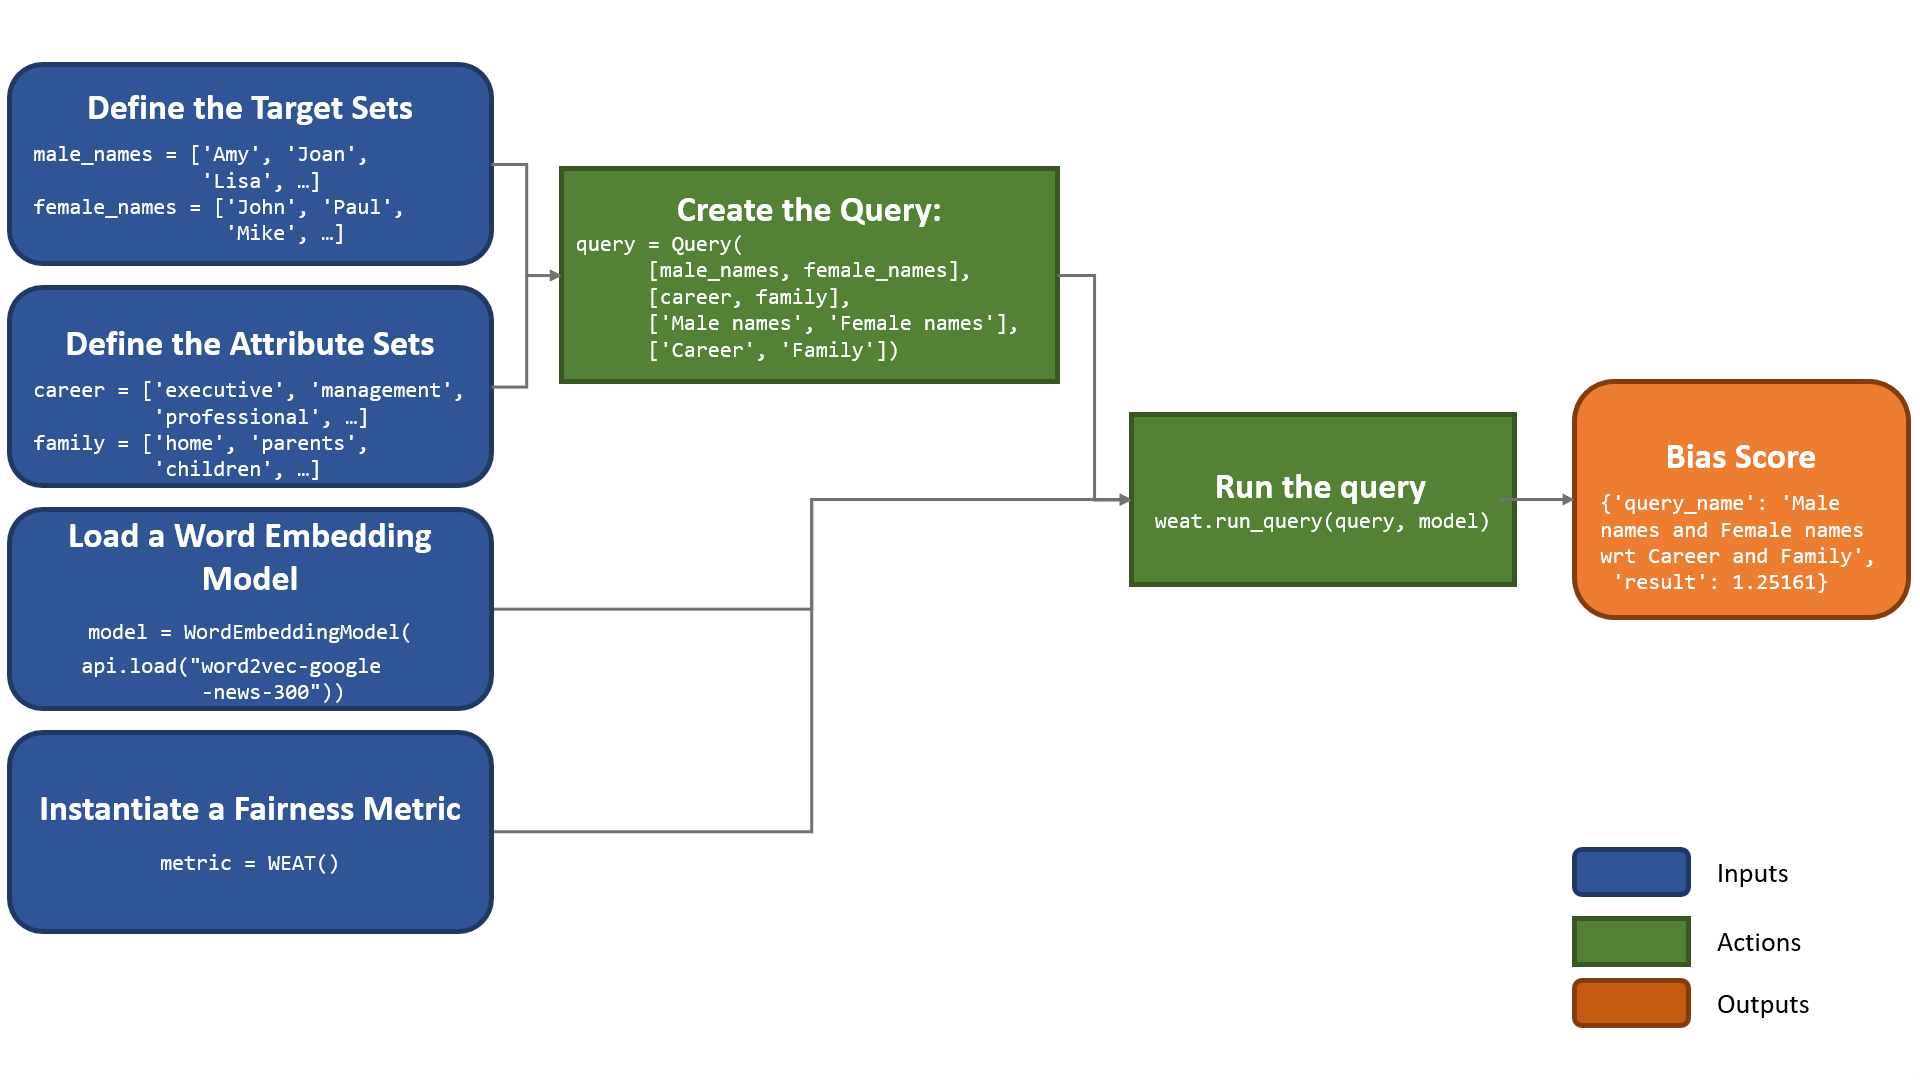
\includegraphics[scale = 0.2]{pics/wefedia.png}
        \end{figure}

\end{scriptsize}
\end{frame}



\begin{frame}{Incremental Word Vectors}
\begin{scriptsize}
\begin{itemize}
 \item An algorithm capable of continuously learning word vectors and thus understanding how the meaning evolves over time (e.g., monitoring the word ``estallido'' in social networks during the Chilean social unrest). \cite{bravo2021incremental}.
\end{itemize}
  \begin{figure}[h]
        	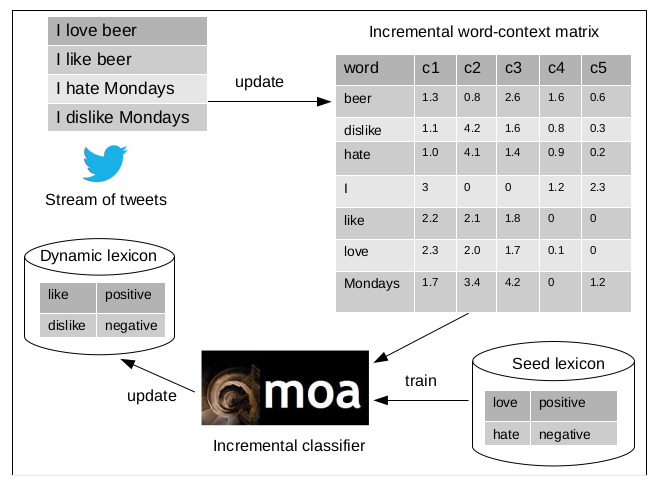
\includegraphics[scale = 0.35]{pics/incdiagram.png}
        \end{figure}

\end{scriptsize}
\end{frame}

\begin{frame}{Incremental Word Vectors}
\begin{scriptsize}
\begin{itemize}
 \item We simulate sentiment change by randomly picking some words and swapping their context with the context of words exhibiting the opposite sentiment.

   \begin{figure}[h]
        	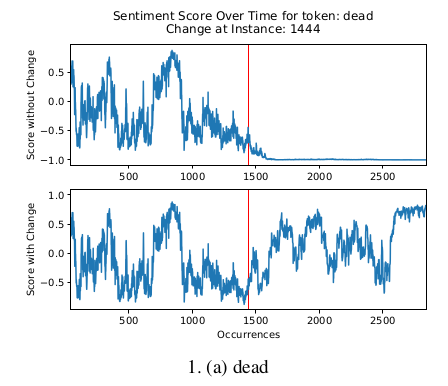
\includegraphics[scale = 0.35]{pics/change.png}
        \end{figure}

 \item Our approach allows for successfully tracking of the sentiment of words over time even when drastic change is induced.

\end{itemize}


\end{scriptsize}
\end{frame}




\begin{frame}{PolyLM: a polysemous language model}
\begin{scriptsize}
\begin{itemize}
 \item A language model capable of automatically learning multiple meanings of a word (e.g. apple:apple, apple:company) \cite{ansell2021polylm}.
\end{itemize}
  \begin{figure}[h]
        	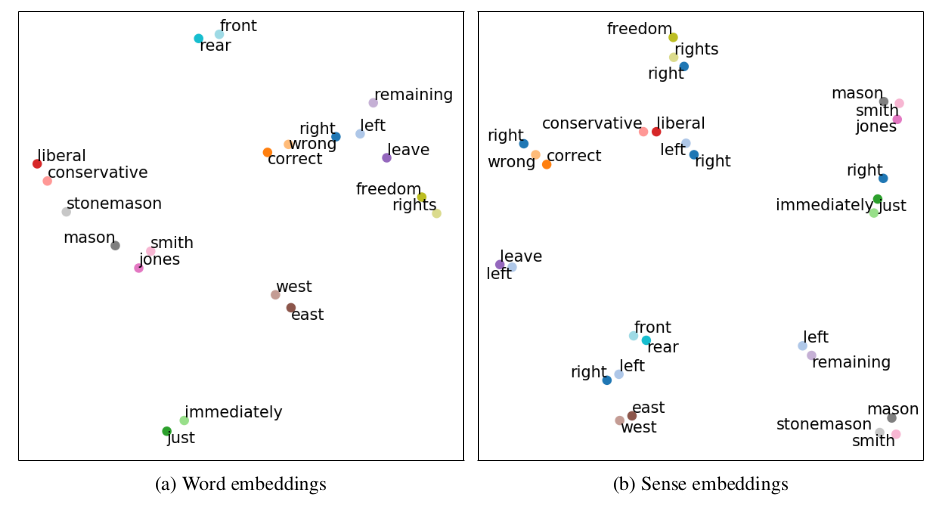
\includegraphics[scale = 0.3]{pics/senseembeddings.png}
        \end{figure}

\end{scriptsize}
\end{frame}



\begin{frame}{PolyLM: a polysemous language model}

  \begin{figure}[h]
        	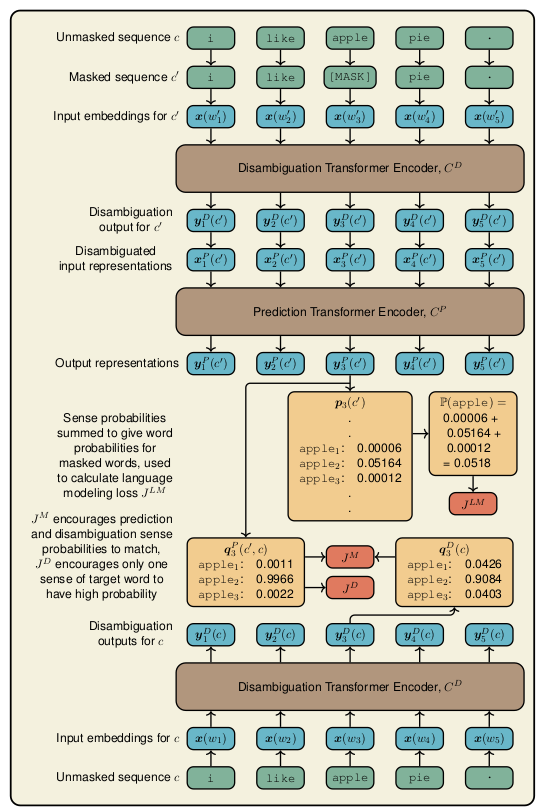
\includegraphics[scale = 0.29]{pics/polylm.png}
        \end{figure}


\end{frame}



\begin{frame}
\frametitle{Questions?}
%\vspace{1.5cm}
\begin{center}\LARGE Thanks for your Attention!\\ \end{center}



\end{frame}

\begin{frame}[allowframebreaks]\scriptsize
\frametitle{References}
\bibliography{bio}
\bibliographystyle{apalike}
%\bibliographystyle{flexbib}
\end{frame}  


%%%%%%%%%%%%%%%%%%%%%%%%%%%

\end{document}
